% abtex2-modelo-artigo.tex, v-1.9.2 laurocesar
% Copyright 2012-2014 by abnTeX2 group at http://abntex2.googlecode.com/ 
%

% ------------------------------------------------------------------------
% ------------------------------------------------------------------------
% abnTeX2: Modelo de Artigo Acadêmico em conformidade com
% ABNT NBR 6022:2003: Informação e documentação - Artigo em publicação 
% periódica científica impressa - Apresentação
% ------------------------------------------------------------------------
% ------------------------------------------------------------------------

\documentclass[
	% -- opções da classe memoir --
	article,			% indica que é um artigo acadêmico
	11pt,				% tamanho da fonte
	oneside,			% para impressão apenas no verso. Oposto a twoside
	a4paper,			% tamanho do papel. 
	% -- opções da classe abntex2 --
	%chapter=TITLE,		% títulos de capítulos convertidos em letras maiúsculas
	%section=TITLE,		% títulos de seções convertidos em letras maiúsculas
	%subsection=TITLE,	% títulos de subseções convertidos em letras maiúsculas
	%subsubsection=TITLE % títulos de subsubseções convertidos em letras maiúsculas
	% -- opções do pacote babel --
	english,			% idioma adicional para hifenização
	brazil,				% o último idioma é o principal do documento
	sumario=tradicional
	]{abntex2}


% ---
% PACOTES
% ---

% ---
% Pacotes fundamentais 
% ---
\usepackage{lmodern}			% Usa a fonte Latin Modern
\usepackage[T1]{fontenc}		% Selecao de codigos de fonte.
\usepackage[utf8]{inputenc}		% Codificacao do documento (conversão automática dos acentos)
\usepackage{indentfirst}		% Indenta o primeiro parágrafo de cada seção.
\usepackage{nomencl} 			% Lista de simbolos
\usepackage{color}				% Controle das cores
\usepackage{graphicx}			% Inclusão de gráficos
\usepackage{microtype} 			% para melhorias de justificação
% ---
		
% ---
% Pacotes adicionais, usados apenas no âmbito do Modelo Canônico do abnteX2
% ---
\usepackage{lipsum}				% para geração de dummy text
% ---
		
% ---
% Pacotes de citações
% ---
\usepackage[brazilian,hyperpageref]{backref}	 % Paginas com as citações na bibl
\usepackage[alf]{abntex2cite}	% Citações padrão ABNT
% ---

% ---
% Configurações do pacote backref
% Usado sem a opção hyperpageref de backref
\renewcommand{\backrefpagesname}{Citado na(s) página(s):~}
% Texto padrão antes do número das páginas
\renewcommand{\backref}{}
% Define os textos da citação
\renewcommand*{\backrefalt}[4]{
	\ifcase #1 %
		Nenhuma citação no texto.%
	\or
		Citado na página #2.%
	\else
		Citado #1 vezes nas páginas #2.%
	\fi}%
% ---

% ---
% Informações de dados para CAPA e FOLHA DE ROSTO
% ---
\titulo{Artigo Traceroute }
\autor{ Rafael Gonçalves de Oliveira Viana}
\local{Brasil}
\data{2017}
% ---

% ---
% Configurações de aparência do PDF final

% alterando o aspecto da cor azul
\definecolor{blue}{RGB}{41,5,195}

% informações do PDF
\makeatletter
\hypersetup{
     	%pagebackref=true,
		pdftitle={\@title}, 
		pdfauthor={\@author},
    	pdfsubject={Modelo de artigo científico com abnTeX2},
	    pdfcreator={LaTeX with abnTeX2},
		pdfkeywords={abnt}{latex}{abntex}{abntex2}{atigo científico}, 
		colorlinks=true,       		% false: boxed links; true: colored links
    	linkcolor=blue,          	% color of internal links
    	citecolor=blue,        		% color of links to bibliography
    	filecolor=magenta,      		% color of file links
		urlcolor=blue,
		bookmarksdepth=4
}
\makeatother
% --- 

% ---
% compila o indice
% ---
\makeindex
% ---

% ---
% Altera as margens padrões
% ---
\setlrmarginsandblock{3cm}{3cm}{*}
\setulmarginsandblock{3cm}{3cm}{*}
\checkandfixthelayout
% ---

% --- 
% Espaçamentos entre linhas e parágrafos 
% --- 

% O tamanho do parágrafo é dado por:
\setlength{\parindent}{1.3cm}

% Controle do espaçamento entre um parágrafo e outro:
\setlength{\parskip}{0.2cm}  % tente também \onelineskip

% Espaçamento simples
\SingleSpacing

% ----
% Início do documento
% ----
\begin{document}

% Retira espaço extra obsoleto entre as frases.
\frenchspacing 

% ----------------------------------------------------------
% ELEMENTOS PRÉ-TEXTUAIS
% ----------------------------------------------------------

%---
%
% Se desejar escrever o artigo em duas colunas, descomente a linha abaixo
% e a linha com o texto ``FIM DE ARTIGO EM DUAS COLUNAS''.
% \twocolumn[    		% INICIO DE ARTIGO EM DUAS COLUNAS
%
%---
% página de titulo
\maketitle

% resumo em português
\begin{resumoumacoluna}
 Este artigo tem como objetivo uma apresentação do funcionamento do Traceroute uma ferramenta de gerenciamento de rede. O traceroute é utilizado para detectar falhas como, por exemplo, gateways intermediários que descartam pacotes ou rotas que excedem a capacidade de um datagrama ip entre outras. Também será de vital importância para esse artigo uma abortagem ao seus protrocolo e o funcionamento dos mesmos.
 
 
 \vspace{\onelineskip}
 
 \noindent
 \textbf{Palavras-chaves}: Roteamento, IP, UDP ,TCP SYN, Ping.
\end{resumoumacoluna}

% ]  				% FIM DE ARTIGO EM DUAS COLUNAS
% ---

% ----------------------------------------------------------
% ELEMENTOS TEXTUAIS
% ----------------------------------------------------------
\textual

% ----------------------------------------------------------
% Introdução
% ----------------------------------------------------------
\section*{Introdução}
\addcontentsline{toc}{section}{Introdução}
A Internet é uma agregação grande e complexa de hardware de rede, conectada entre eles por gateways. Seguir a rota que os pacotes seguem (ou encontrar o gateway que está descartando seus pacotes) pode ser difícil. 
Nesse artigo estaremos abortando o Trouceroute porém, será levantado protolocos que o trouceroute utiliza para seu funcionamento porém muito breve.

\section{Protocolos}

\subsection{IPv4}
O IP é o elemento comum encontrado na Internet pública dos dias de hoje. É descrito no RFC 791 da IETF, que foi pela primeira vez publicado em Setembro de 1981. Este documento descreve o protocolo da camada de rede mais popular e atualmente em uso. Esta versão do protocolo é designada de versão 4, ou IPv4. O IPv6 tem endereçamento de origem e destino de 128 bits, oferecendo mais endereçamentos que os 32 bits do IPv4.

Ente os 12 campos do IPv4 descrito no RFC 791 falaremos do TTL é campo de oito bits, o TTL (time to live, ou seja, tempo para viver) ajuda a prevenir que os datagramas persistam (ex. andando aos círculos) numa rede. Historicamente, o campo TTL limita a vida de um datagrama em segundos, mas tornou-se num campo de contagem de nós caminhados. Cada comutador de pacotes que um datagrama atravessa decrementa o campo TTL em um valor. Quando o campo TTL chega a zero, o pacote não é seguido por um comutador de pacotes e é descartado.
O propósito do TTL é evitar que datagramas entrem em um loop de roteamento, o que pode ocorrer devido a algum tipo de falha durante o roteamento dos pacotes. Quando um roteador recebe um datagrama cujo TTL é igual a 0 (zero), ele não o encaminhará mais. Em vez disso, o roteador irá descartar o pacote e enviar de volta ao host que o originou uma mensagem ICMP do tipo Tempo Excedido. Essa mensagem contém o endereço IP do roteador como endereço de origem - e esse é o segredo do traceroute.\cite{boson}

\subsection{ICMP}

O protocolo ICMP (Internet Control Message Protocol - Protocolo de Mensagens de Controle de Internet) é um protocolo que permite gerenciar as informações relativas aos erros nas máquinas conectadas. Devido aos poucos controles que o protocolo IP realiza, ele não corrige estes erros mas os mostra para os protocolos das camadas vizinhas. Assim, o protocolo ICMP é usado por todos os roteadores para assinalar um erro, chamado de Delivery Problem ou, em português, Problema de Entrega. 

O ICMP é um protocolo integrante do Protocolo IP, definido pela RFC 792, e utilizado para fornecer relatórios de erros ao host que deu origem aos pacotes enviados na rede. Qualquer computador que utilize o protocolo IP precisa aceitar as mensagens ICMP e alterar o seu comportamento de acordo com o erro relatado.

Os gateways (roteadores) devem também estar programados para enviar mensagens ICMP quando receberem pacotes que provoquem algum tipo de erro ou detectarem algum problema listado no protocolo ICMP. O ICMP é transportado no campo de dados do pacote IP e identificado como tipo de protocolo “1” pelo cabeçalho do IP.

As principais mensagens de erro ou informacionais do ICMP geralmente são enviadas automaticamente em uma das seguintes situações:

Um pacote IP não consegue chegar ao seu destino, por exemplo, quando o tempo de vida (TTL) do pacote está expirado (o contador chegou à zero). Esta mensagem é o tempo de vida expirado ou “time exceeded”.

O roteador não consegue retransmitir os pacotes na frequência adequada, ou seja, o roteador está congestionado (mensagem “source quench”).

O roteador indica uma rota melhor para o host que está enviando pacotes (mensagem de redirecionamento de rota ou “redirect”).

Quando um host de destino ou rota não está alcançável (mensagem “destination unreachable” ou destino inalcançável).

Quando o host ou o roteador descobrem um erro de sintaxe no cabeçalho do IP (mensagem “parameter problem”). 

Existem diversas outras mensagens que o ICMP pode fornecer e cada uma é representada por um tipo ou código.\cite{dltec}

\subsection{Recuo do ambiente }



\section{Traceroute}
O utilitário traceroute, que foi escrito por Van Jacobson em 1987, é uma ferramenta de diagnóstico que nos permite ver a rota que datagramas IP seguem quando são enviados de um host a outro. O traceroute faz uso do protocolo ICMP e do campo TTL no cabeçalho IP do datagrama. O valor a ser usado neste campo varia entre os sistemas operacionais, sendo comuns os valores 128 para sistemas Windows e 64 para sistemas baseados em Unix, como o Linux (em pacotes normais; o traceroute utiliza valores totalmente diferentes).

\subsection{Funcionamento}
Traceroute utiliza o campo TTL "time to live" do protocolo IP e tenta obter uma resposta ICMP TIME\_EXCEEDED de cada gateway ao longo do caminho para algum host.
Toda vez que um datagrama chega a um roteador, seu TTL é decrementado em um antes de ser encaminhado adiante. O propósito do TTL é evitar que datagramas entrem em um loop de roteamento, o que pode ocorrer devido a algum tipo de falha durante o roteamento dos pacotes. Quando um roteador recebe um datagrama cujo TTL é igual a 0 (zero), ele não o encaminhará mais. Em vez disso, o roteador irá descartar o pacote e enviar de volta ao host que o originou uma mensagem ICMP do tipo Tempo Excedido. Essa mensagem contém o endereço IP do roteador como endereço de origem - e esse é o segredo do traceroute.\cite{boson}
SINTAXE

\subsection{Comandos Traceroute}

traceroute [-m Max\_ttl] [-n] [-p Port] [-q Nqueries] [-r] [-s SRC\_Addr]

[-t TypeOfService] [-v] [-w WaitTime] Host [PacketSize]

O único parâmetro obrigatório para o comando traceroute é o nome ou o número IP do host destino. O tamanho do pacote UDP (UDP probe packet) é de 38 bytes, mas pode ser aumentado especificando o tamanho do pacote (em bytes) após o nome ou número IP do destino.



\subsubsection{Opções}



\subitem{-m Max\_ttl}

Especifica um "time-to-live" máximo (número máximo de hops) usado nos pacotes de pesquisa UDP. O default é  30 hops  (o mesmo dafault utilizado para conexões TCP).

-n         

Mostra o endereço IP de cada gateway encontrado no caminho (da origem ao destino).



-p Port    

Especifica o número base da porta UDP utilizada na pesquisa do traceroute. O default é 33434. O comando traceroute depende de um intervalo de portas UDP abertas de "base a base + número de hops - 1" no host destino. Se uma porta UDP não está disponível, esta opção pode ser usada para pegar um intervalo de portas não utilizadas.

-q Nqueries 

Especifica o número de pacotes UDP (UDP probes) que o comando traceroute envia a cada Max\_ttl. O default é três pacotes.

-r           

Desvia das tabelas de roteamento e envia os pacotes de pesquisa diretamente a um host. Se este host não está na rede, um erro é retornado. Esta opção pode ser usada para "dar" um comando ping em um host local através de uma interface que não está registrada nas tabelas de roteamento.



-s SRC\_Addr

Usa o endereço especificado (SRC\_Addr) como o endereço de origem dos pacotes UDP enviados. Em hosts com mais de um endereço IP, a opção "-s" pode ser usada para forçar o endereço de origem a ser uma interface específica e não, necessariamente, aquela de onde o pacote foi enviado. Se o endereço IP especificado não for válido, um erro é retornado e nada é enviado.

-t TypeOfService

Atribui um valor entre 0 e 255 para a variável TypeOfService do pacote de pesquisa UDP. O default é 0 (zero). Esta opção pode ser utilizada para descobrir se diferentes tipos de serviços resultam em diferentes caminhos.

-v        

Recebe pacotes diferentes de TIME-EXCEEDED e PORT-UNREACHABLE.



-w WaitTime 

Especifica o tempo (em segundos) a esperar pela resposta a um pacote de pesquisa UDP. O default é 3 segundos.

Host      

Especifica o host destino, pelo nome ou pelo seu número IP. Este parâmetro é obrigatório. PacketSize Especifica o tamanho (em bytes)  do pacote UDP de pesquisa (probe). O default é 38 bytes.                  


\subsubsection{Linux x Windows}
O valor a ser usado neste campo varia entre os sistemas operacionais, sendo comuns os valores 128 para sistemas Windows e 64 para sistemas baseados em Unix, como o Linux (em pacotes normais; o traceroute utiliza valores totalmente diferentes).
\subsubsection{Comandos}

\section{Exemplo de reconhecimento de cumutação de rede utilizando Traceroute}
A cumutação de pacotes que a Internet utiliza visa percorrer os melhores caminhos possíveis, sendo assim lentidão na rede ocasionada por diversos problemas, se possivel consultar Kurrose 2010 para melhores exemplos de problemas originadores de lentidão na rede, o exemplo dado nesse artigo tem como objetivo demostrativo com intuito de analizar mensagens ICMP relatadas pelo Traceroute, e mapear essas mensagens utilizando os ips disponíveis nas respostas do Traceroute, com auxilio da pagína www.localizaip.com.br, que nos fornece posições geograficas, com essas informações geograficas (latitude e longitude) foram meapeado utilizando o aplicativo Google Earth . 

\subsubsection{Reconhecimento}
Primeiramente foi 
\begin{figure}[!htb]
	\centering
	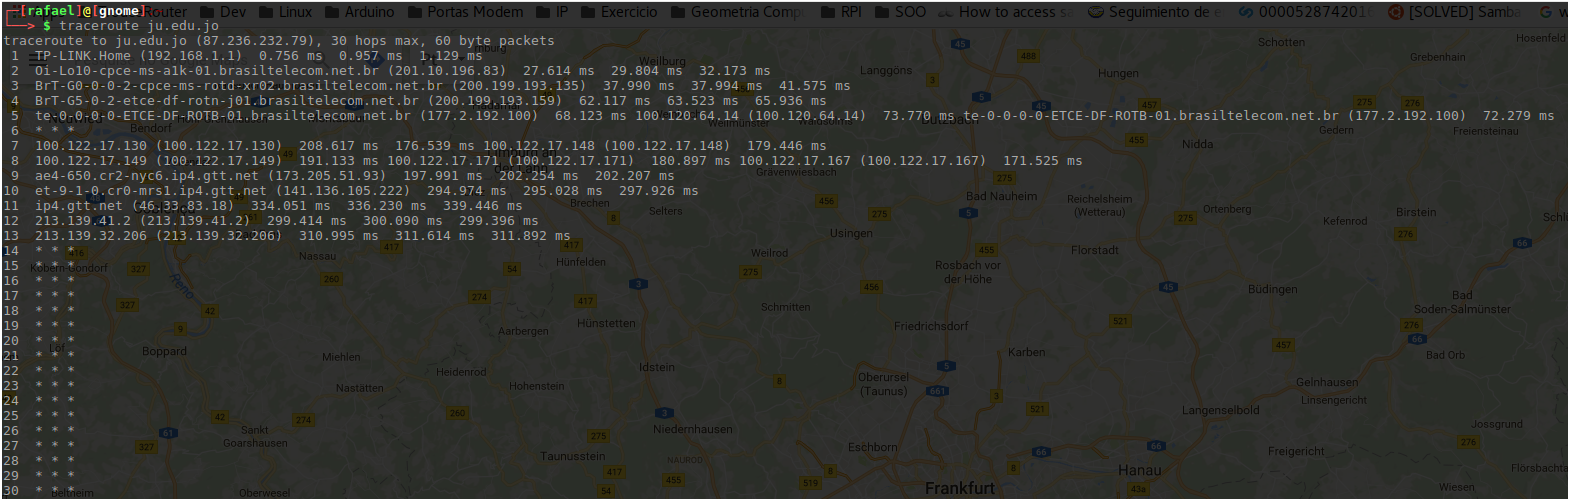
\includegraphics[scale=0.3]{./trauceroute-1.png}
	\caption{}
	\label{Rotulo}
\end{figure}

\subsubsection{Levantamento de rotas}

\subsubsection{Mapeamento Utilizando Google Eart }

\begin{figure}[!htb]
	\centering
	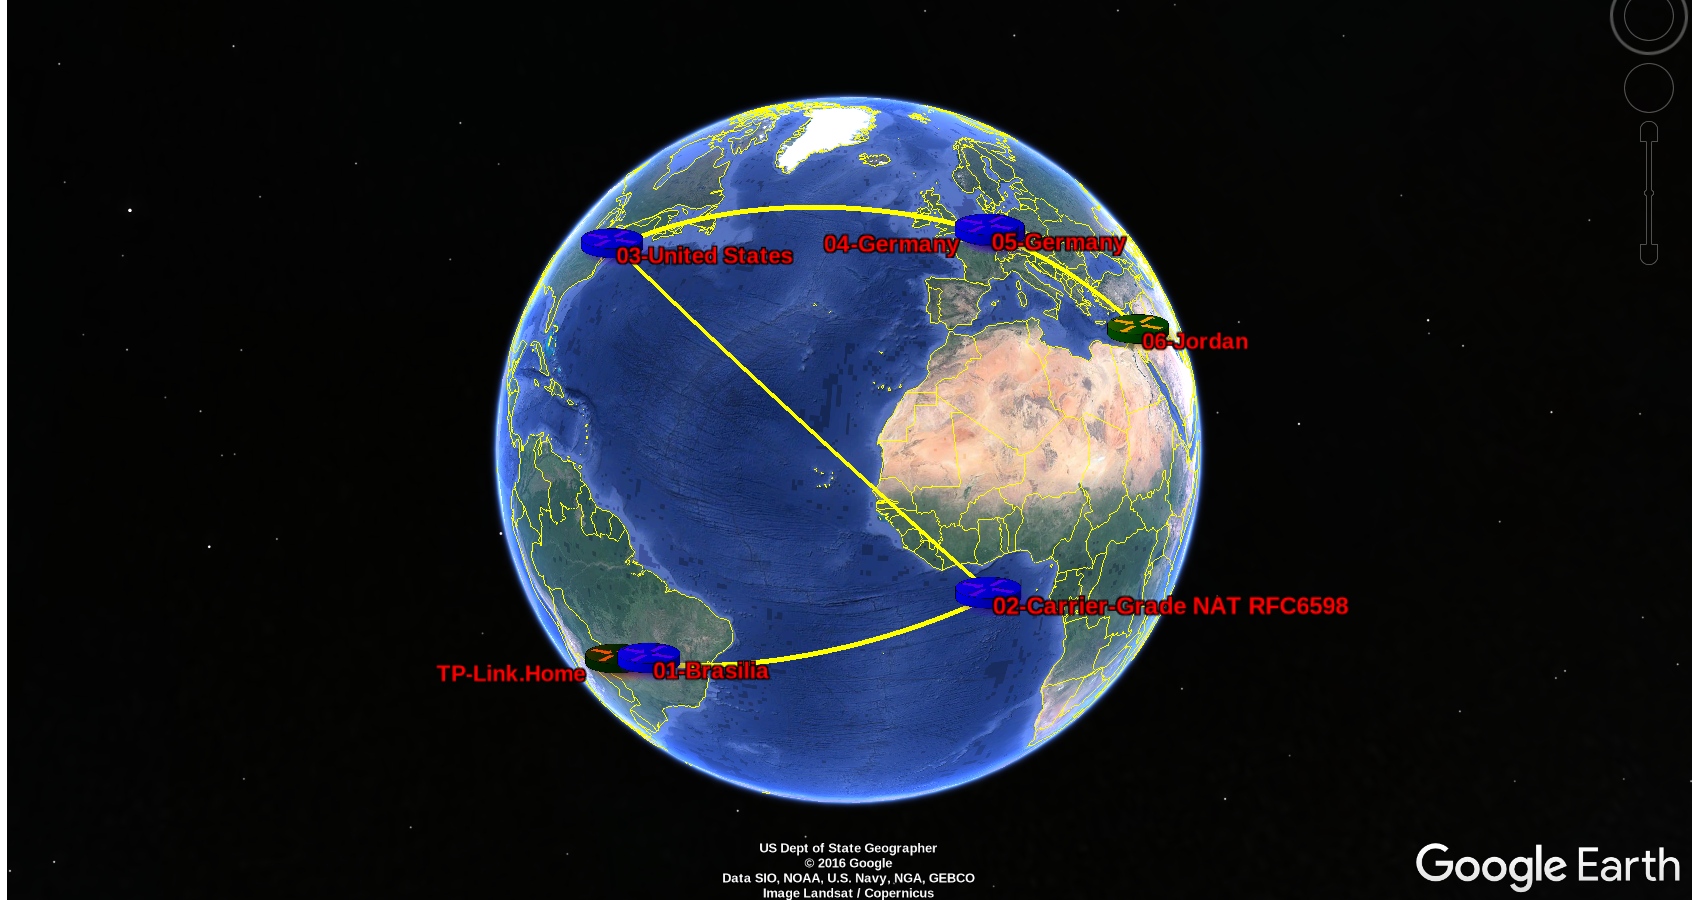
\includegraphics[scale=0.2]{./google-earh.png}
	\caption{}
	\label{Rotulo}
\end{figure}

\section{Mais exemplos no Modelo Canônico de Trabalhos Acadêmicos}

Este modelo de artigo é limitado em número de exemplos de comandos.


\section{Consulte o manual da classe \textsf{abntex2}}


% ---
% Finaliza a parte no bookmark do PDF, para que se inicie o bookmark na raiz
% ---
\bookmarksetup{startatroot}% 
% ---

% ---
% Conclusão
% ---
\section{Considerações finais}
\addcontentsline{toc}{section}{Considerações finais}

\lipsum[1]

\begin{citacao}
\lipsum[2]
\end{citacao}

\lipsum[3]
\bibliographystyle{abntex2-alf}
\bibliography{abntex2-modelo-references}



\end{document}
